\documentclass[a4paper,10pt]{ltjsarticle}

\usepackage[margin=22mm]{geometry}
\usepackage{amsmath,amssymb}
\usepackage{booktabs}
\usepackage{float}
\usepackage{graphicx}
\usepackage{natbib}
\usepackage{tikz}
\usepackage{xcolor}
\usepackage{hyperref}
\usepackage{listings}
\usetikzlibrary{positioning}

\hypersetup{
  unicode=true,
  colorlinks=true,
  linkcolor=blue!55!black,
  citecolor=blue!55!black,
  urlcolor=blue!55!black,
  pdftitle={MassivelyによるGPU SPH：セルグラフと入れ子のSegmentIteratorによる動的近傍の表現},
  pdfauthor={Akira Hayakawa},
  pdfsubject={GPU SPHの実装課題とMassively v0.80による解決}
}
\graphicspath{{../workspace/plot/}}
\newcommand{\code}[1]{\texttt{#1}}
\newcommand{\Seg}{\operatorname{Seg}}
\newcommand{\Perm}{\operatorname{Permute}}
\lstset{
  basicstyle=\ttfamily\small,
  frame=single,
  columns=fullflexible,
  keepspaces=true,
  breaklines=true,
  showstringspaces=false
}

\title{MassivelyによるGPU Smoothed Particle Hydrodynamics：\\
セルグラフと入れ子のSegmentIteratorによる動的近傍の表現}
\author{Akira Hayakawa}
\date{2026年7月18日}

\begin{document}
\maketitle

\begin{abstract}
GPU上にSmoothed Particle Hydrodynamics（SPH）を実装する際の中心的な困難は、
粒子対の式自体ではなく、移動し長さが一定でない近傍である。本稿では、このworkloadを
Massively v0.80のiterator algebraでどのように表現したかを説明する。一様格子セルの
隣接関係をcompressed sparse row（CSR）グラフとして一度だけ保存する。導関数を評価する
たびに粒子状態をセル順にsortし、lower boundによりセルから粒子への第2のCSR分割を作る。
続いて、遅延permutationと2層の\code{SegmentIterator}により、両者をquery粒子ごとの
segment-of-segmentsへ合成する。\code{Segment}はコピーされた近傍データではなく境界を
GPU値として持つread-onlyな意味的viewであるため、大域的な粒子対リストは実体化されない。
1回のtransform invocationが1個のquery粒子を所有し、すべての寄与をprivateなaccumulatorへ
gatherするので、atomic演算とwrite conflictを必要としない。また、Massivelyの型レベル上限で
ある13個のread leafを満たすため、solverをどのように分解したかを示す。end-to-endの物理的な
確認にはSod shock tubeを用い、$t=0.15$におけるsample密度の$L_1$誤差は0.004199となった。
65,536粒子では、GPU密度とCPU全粒子対referenceの最大相対差は
$5.89\times10^{-6}$であった。内蔵Radeon 680Mでは、完全な2次元密度snapshotが
5.109 msであり、CPU cell-list計算の16.204 msに対して高速であった。以上は新しいSPH
離散化の提案ではなく、SPHを型付きGPU iterator systemへ写像する際の障害を特定し、
Massivelyによる対応する構成を示し、その利点と費用を測定する実装研究である。
\end{abstract}

\section{はじめに}

Smoothed Particle Hydrodynamicsは、Euler格子を移動粒子とcompact supportを持つ補間kernelで
置き換える\citep{gingold1977,monaghan1992}。粒子$i$について、密度、圧力、人工粘性は
近傍粒子に関する和である。数値式は$i$について自然に並列化できるが、寄与する粒子集合は
粒子が動くたびに変化する。そのためGPU実装では、位置から不揃いな近傍関係を繰り返し構築し、
同時に効率的な状態アクセスと有界なmemory使用量を維持しなければならない。

従来のGPU SPH実装では、この問題をsort済みcell list、linked cell、Verlet list、または
専用の相互作用kernelにより解決している
\citep{herault2010,dominguez2011,dominguez2013,winkler2018}。Massivelyは異なるprogramming
手段を提供する。CubeCL上に、device algorithmとlogical iteratorの型付きalgebraを提供する
\citep{massively080,cubecl}。zip、transform、permutation、segmentationを合成し、実行を伴う
algorithmがその式をGPU kernelへloweringする。本研究の問いは次のように明確化できる。

\begin{quote}
粒子ごとに近傍リストを実体化せず、移動するSPH近傍をMassively iteratorとしてどう表現するか。
また、完全なsolverに残るGPU上の制約をどう処理するか。
\end{quote}

本稿の貢献は以下である。
\begin{itemize}
  \item 静的なセルCSR、動的に再構築するセル--粒子分割、遅延permutation、および入れ子の
        segmented iterationを合成してSPH近傍を得る方法を明示的に導出した。
  \item 各GPU invocationが1個のquery粒子を評価して1個の出力を書くrace-freeなgather形式を
        示し、そのmemory量と計算量のtrade-offを明らかにした。
  \item Massively v0.80のread arity上限13のもとで、1次元・2次元の密度、圧力、仕事、および
        粘性kernelをfield単位でどう分解するかを示した。
  \item 構造テストとdifferential test、Sod shock tube、および密度pipeline benchmarkによる
        検証結果を示した。
\end{itemize}

本実装は固定平滑化長、cubic spline、一次精度時間積分、および人工粘性を用いる。
end-to-endの物理検証には標準的なSod shock tubeを用いる。

\section{SPHが突きつける実装上の問題}

\subsection{粒子対workload}

粒子の位置$\mathbf{x}_i$、速度$\mathbf{v}_i$、質量$m_i$、密度$\rho_i$、比内部エネルギー
$e_i$、および平滑化長$h$について、実装した密度推定は
\begin{equation}
  \rho_i = \sum_j m_j W_d(\lVert\mathbf{x}_i-\mathbf{x}_j\rVert,h)
  \label{eq:density-ja}
\end{equation}
である。理想気体の状態方程式は$p_i=(\gamma-1)\rho_i e_i$である。圧力と粘性の導関数は
一般に次のSPH形式を持つ。
\begin{align}
  \frac{d\mathbf{v}_i}{dt}
    &= -\sum_j m_j\left(\frac{p_i}{\rho_i^2}
                       +\frac{p_j}{\rho_j^2}+\Pi_{ij}\right)
       \nabla_i W_{ij}, \\
  \frac{de_i}{dt}
    &= \sum_j m_j\frac{p_i}{\rho_i^2}
       (\mathbf{v}_i-\mathbf{v}_j)\mathbin{\cdot}\nabla_iW_{ij}
       +\frac12\sum_jm_j\Pi_{ij}
       (\mathbf{v}_i-\mathbf{v}_j)\mathbin{\cdot}\nabla_iW_{ij}.
  \label{eq:derivatives-ja}
\end{align}
これらは標準的な保存型SPHの形式である\citep{monaghan2005,price2012}。実装ではcubic
B-spline
\begin{equation}
 W_d(r,h)=\frac{\sigma_d}{h^d}
 \begin{cases}
  1-\tfrac32q^2+\tfrac34q^3,&0\le q<1,\\
  \tfrac14(2-q)^3,&1\le q<2,\\
  0,&q\ge2,
 \end{cases}
 \qquad q=r/h
 \label{eq:kernel-ja}
\end{equation}
を用いる。ここで$\sigma_1=2/3$、$\sigma_2=10/(7\pi)$である。したがって、粒子対が寄与する
のは$r<2h$の場合だけである。

人工粘性は接近する粒子についてのみ評価する。無次元座標
$\mathbf{q}_{ij}=(\mathbf{x}_i-\mathbf{x}_j)/h$を用いると、実装は係数形式
\begin{equation}
 \mu_{ij}=\frac{(\mathbf{v}_i-\mathbf{v}_j)\cdot\mathbf{q}_{ij}}
                 {\lVert\mathbf{q}_{ij}\rVert^2+0.01},\qquad
 \Pi_{ij}=\frac{-A\mu_{ij}+B\mu_{ij}^2}{\widehat\rho_{ij}}
 \label{eq:viscosity-ja}
\end{equation}
を持つ。1次元では係数を設定可能とし、密度の算術平均を用いる。現在の2次元workloadでは
$A=1$、$B=2$、$\widehat\rho_{ij}=\sqrt{\rho_i\rho_j}$である。この数値的な選択自体は本稿の
貢献ではない。ただし、その因数分解はMassivelyのread arity制約内で演算を表現するため、
後に重要となる。

式\eqref{eq:density-ja}--\eqref{eq:derivatives-ja}からGPU workloadの特徴が分かる。出力粒子
ごとに候補近傍数が異なり、各候補についてquery側とneighbor側の複数columnを必要とする。
また同じ空間関係を、異なるcolumn tupleを用いて密度、圧力、粘性で再利用する。

\subsection{同時に満たすべき5つの条件}

実装は次の5条件を同時に満たす必要がある。
\begin{enumerate}
  \item \textbf{完全で動的な近傍。} 任意に粒子が移動した後も、support内の全粒子対を
        $O(N^2)$ scanなしで訪問しなければならない。
  \item \textbf{整合した並べ替え。} 位置だけをsortし、速度、質量、energy、粒子identityを
        sortしなければ、異なる粒子の状態を気付かずに混合してしまう。
  \item \textbf{race-freeな集約。} 対称な粒子対演算で$i$と$j$の両方を更新すると、GPU上で
        atomic演算またはcoloringが必要になる。
  \item \textbf{有界な表現。} 全候補粒子対の実体化は、粒子ごとの候補数の総和に比例する
        memoryを追加し、粒子移動後に再構築しなければならない。
  \item \textbf{表現可能なkernel。} 合成した入力は、Massively v0.80が扱える静的iterator型と
        kernel read arityに収まらなければならない。
\end{enumerate}
粒子データをdevice上に保持することも実用上の条件である。そうしなければ、正しい近傍kernelを
実装しても、各time stepの転送時間が支配的になり得る。

\section{solverで使用するMassivelyの機構}

\subsection{logical iteratorと実行点}

Massivelyはlogicalな入力式と、allocationおよび実行を伴うalgorithmを区別する。device vectorの
sliceはiteratorであり、\code{zip}はcolumnを結合し、\code{lazy::transform}はindexから読む値を
変換し、\code{lazy::permute(values, indices)}は\code{values[indices[i]]}を読む。これらの式は、
それ自体では結果arrayを作らない。\code{vector::transform}、\code{vector::sort\_by\_key}、
\code{vector::lower\_bound}のようなoperationが、device storageを生成する実行点である。

この区別が設計の中心となる。solverは、大域的に変化する必要があるdata、すなわちsort済み粒子
column、cell ID、cell offset、物理量の出力を実体化する。一方、それらarray間の関係は遅延reader
として表現する。

\subsection{SegmentIteratorが表すもの}

logicalな値stream $V$とoffset $P=(P_0,\ldots,P_K)$について、Massivelyは
\begin{equation}
 \Seg(V,P)[k] = V[P_k:P_{k+1})
 \label{eq:segment-ja}
\end{equation}
を定義する。この\code{SegmentIterator}のitem型は\code{Segment<V::Item>}である。
\code{Segment}は所有権を持つvectorではなく、allocation機能もwrite機能も持たない。生成される
GPU値では、registerに保持される\code{start}と\code{len}の境界だけがsegmentごとに異なる。
backing readerは、その式の全segmentが共有するcompiler側のcontextである。CubeCL operationの
内部では、\code{len()}が動的な長さを返し、\code{at(k)}がbacking expressionの
\code{start + k}からのreadを生成する。

SPHにとって重要な帰結が2つある。第1に、粒子dataをコピーせずsegmentをpermuteできる。第2に、
あるsegment iteratorの値自体をsegmentにでき、外側の\code{Segment}のitemを内側の
\code{Segment<ParticleFields>}にできる。これは「近傍セルと、それぞれの近傍セル内の粒子」を
表すために必要な型そのものである。

\subsection{read arityの境界}

Massivelyはcanonicalな入力式に型レベルのread arityを割り当てる。v0.80で利用可能なarityは
$A_1,\ldots,A_{13}$であり、型レベルの加算は合計が13以下の場合にのみ定義される。この仕組みに
より過大な合成をcompile timeで検出できるが、物理的には自然な単一のSPH式を表現できない場合も
ある。Section~\ref{sec:whole-solver-ja}では、同じ近傍viewを保ちながら実装をどう分割するかを示す。

\section{移動する近傍の構築}

\subsection{静的セルグラフ}

cell幅をcompact support半径と等しい$s=2h$とする。1次元では各cellは自分自身と最大2つの隣接
cellに接続する。2次元では、domain境界で切り取られた$3\times3$ blockに接続する。この関係は
domainの幾何形状に依存するが粒子位置には依存しないため、一度だけCSRとして構築する。
\begin{align}
 A &= (A_0,\ldots,A_{E-1}) &&\text{近傍cell ID},\\
 G &= (G_0,\ldots,G_C) &&\text{row offset},\\
 \mathcal{G}(c) &= A[G_c:G_{c+1}).
\end{align}
$C$個のcellに対し、1次元では$E\le3C$、2次元では$E\le9C$である。

このgraphはkernel supportに対して完全である。
$\lVert\mathbf{x}_i-\mathbf{x}_j\rVert<2h=s$なら、各座標方向の絶対変位も$s$未満である。
したがって整数cell座標の差は各次元で高々1であり、CSR rowは該当する全cell offsetを列挙する。
2次元の$3\times3$ blockの角にあり、円形supportの外にある候補は、粒子対loop内の
式\eqref{eq:kernel-ja}により除外する。

\subsection{動的なセル--粒子分割}

導関数を評価するたびに、Massivelyの\code{vector::transform}で各位置をclamp済みrow-major
cell ID $c_i$へ写像する。その後、structure-of-arraysの完全な状態をzipした値に対して、1回の
\code{sort\_by\_key}を実行する。tupleのfield数は1次元で8、2次元で10である。tuple全体を一度に
sortすることで、次の不変条件を保つ。
\begin{equation}
  (\mathrm{id},\mathbf{x},\mathbf{v},e,m,\text{事前計算した質量因子})_k
  \quad\text{はすべて同じ粒子に属する。}
\end{equation}
sort済みcell keyも、並べ替えた状態とともに保持する。

全cell ID $0,\ldots,C$について、\code{vector::lower\_bound}でsort済みkeyを検索する。その出力
$P=(P_0,\ldots,P_C)$が粒子streamを分割する。
\begin{equation}
 \mathcal{B}(c)=V[P_c:P_{c+1})
 \label{eq:cell-particles-ja}
\end{equation}
空cellに特別な処理は不要であり、単に$P_c=P_{c+1}$となる。

\subsection{入れ子segmentへの合成}

中心となる構成をRust型から独立に記述する。$V$を、粒子のsort順に並んだ任意のneighbor fieldの
zip streamとする。次を定義する。
\begin{align}
 B &= \Seg(V,P),
   & B[c] &= \mathcal{B}(c),\\
 R &= \Perm(B,A),
   & R[e] &= B[A_e],\\
 H &= \Seg(R,G),
   & H[c] &= (B[A_{G_c}],\ldots,B[A_{G_{c+1}-1}]),\\
 N &= \Perm(H,c),
   & N[i] &= H[c_i].
 \label{eq:nested-ja}
\end{align}
したがって$N[i]$はquery粒子$i$について、cell segmentを要素とするsegmentである。型変換を省略
したMassivelyの実際のpatternをListing~\ref{lst:nested-ja}に示す。

\begin{lstlisting}[caption={1個のSPH近傍viewを構築するMassivelyコードの概略。},label={lst:nested-ja}]
let b = SegmentIterator::new(values, particle_offsets);
let r = lazy::permute(b, neighbor_cells);
let h = SegmentIterator::new(r, graph_offsets);
let n = lazy::permute(h, cell_ids);
let output = vector::transform(exec, zip(query, n), PairReduction)?;
\end{lstlisting}

第1の\code{SegmentIterator}は、実体化されたsort済みcolumnとparticle offsetをbacking dataとする。
$A$によるpermutation、$G$による第2のsegmentation、$c_i$による最後のpermutationは、logicalな
read expressionのままである。特に、全$(i,j)$粒子対を格納するarrayも、各$i$の近傍vectorを
コピーしたarrayも存在しない。入れ子viewに必要な物理的topology入力は$P$、$A$、$G$、$c$だけで
ある。

\begin{figure}[H]
  \centering
  \resizebox{\textwidth}{!}{%
  \begin{tikzpicture}[
      node distance=8mm and 8mm,
      box/.style={draw,rounded corners,align=center,minimum height=9mm,fill=blue!5},
      view/.style={draw,rounded corners,align=center,minimum height=9mm,fill=green!8},
      arrow/.style={-latex,thick}]
    \node[box] (state) {device常駐の\\粒子SoA状態};
    \node[box,right=of state] (key) {cell ID\\transform};
    \node[box,right=of key] (sort) {zip済み状態の\\sort};
    \node[box,right=of sort] (offset) {cell offsetの\\lower bound};
    \node[view,right=of offset] (nested) {遅延評価される入れ子\\segment view};
    \node[box,right=of nested] (reduce) {query粒子ごとの\\1出力};
    \node[box,below=of nested] (graph) {静的cell CSR\\$A,G$};
    \draw[arrow] (state)--(key);
    \draw[arrow] (key)--(sort);
    \draw[arrow] (sort)--(offset);
    \draw[arrow] (offset)--(nested);
    \draw[arrow] (sort) to[bend left=20] (nested);
    \draw[arrow] (graph)--(nested);
    \draw[arrow] (nested)--(reduce);
  \end{tikzpicture}}
  \caption{青は実体化されるstage、緑は遅延viewである。粒子所属を再構築しても、静的cell graphは
  再構築しない。}
  \label{fig:neighborhood-ja}
\end{figure}

\subsection{race-freeなgatherとcost}

最後の\code{vector::transform}はquery粒子ごとに1個のlogical operationを起動する。そのoperationは
外側のcell segmentと内側のparticle segmentを走査し、$q\ge2$を除外し、operation localな
CubeCL \code{RuntimeCell}へ集約する。invocation $i$は出力$i$だけを書く。他の粒子の導関数を
書くinvocationはないため、atomic additionも粒子対coloringも必要ない。

意図したtrade-offとして、相互作用するunordered pairは通常2回評価される。すなわち
$i\mathbin{\to}j$と$j\mathbin{\to}i$である。scatter形式なら粒子対の算術演算を再利用できるが、
同期問題が再び生じる。ここでは、単純なownership ruleと連続したquery出力を優先してgather形式を
採用する。

$Q$をcell rowが列挙するordered candidate interactionの個数とする。保存する表現は
$O(N+C+E)$であり、永続的な候補listの$O(N+Q)$とは異なる。1回のprepareは
\begin{equation}
 T_{\mathrm{prepare}}=
 T_{\mathrm{sort}}(N)+O(N)+O(C\log N)+O(Q)
 \label{eq:cost-ja}
\end{equation}
のwork modelを持つ。$T_{\mathrm{sort}}$はbackend依存のままとし、$C+1$個のlower-bound queryが
$O(C\log N)$項に対応する。cell占有数が有界なら$Q=O(N)$である。この解析は、不揃いなsegment長に
よるdivergenceを消去するものではない。Massivelyは表現とloweringの仕組みを提供するが、実行する
work量は物理的な粒子分布に依存する。

\section{完全なsolverへの写像}
\label{sec:whole-solver-ja}

\subsection{device常駐pipeline}

粒子identity、位置、速度、比内部エネルギー、質量、および$m/h$の冪をstructure-of-arrays形式の
device vectorへuploadする。1 stepでは次を実行する。
\begin{enumerate}
  \item cell IDを計算し、完全なzip済み状態をsortし、particle offsetを得る。
  \item 位置を$h^{-1}$でscaleし、入れ子近傍を通して密度を評価する。
  \item 理想気体の状態方程式をelementwiseに評価する。
  \item 同じsort済み粒子に対して圧力、圧力仕事、粘性用の型付きviewを再構築し、それぞれの
        粒子対reductionを評価する。
  \item 導関数を合成し、energy、速度、位置を更新する。
  \item 次stepのため新しいarrayをdeviceに保持する。
\end{enumerate}
明示的なdevice-to-host転送を行うのは\code{snapshot}だけである。sortによりstorage順が変わるため、
snapshotは安定した粒子IDを含む。必要であれば、device外で物理出力をidentity順へ戻せる。

各物理operatorが必要とするneighbor tupleは異なるため、同じ空間近傍であっても型付きviewを
operatorごとに再構築する。密度は位置と質量因子を読み、圧力はさらに$p/\rho^2$を読み、粘性は
速度と密度因子を読む。これらのviewは、実体化済みの$P$、$A$、$G$、$c$を共有する。

\subsection{13個のread leafに収める方法}

Table~\ref{tab:arity-ja}は、合成された各入力の物理的leaf数を示す。4個のtopology leafは、particle
offset $P$、neighbor cell ID $A$、cell graph row offset $G$、query cell ID $c$である。残りが
query columnとneighbor columnである。

\begin{table}[ht]
  \centering
  \caption{Massively v0.80におけるread arityの分解。}
  \label{tab:arity-ja}
  \begin{tabular}{lrrrr}
    \toprule
    operation & query field & neighbor field & topology & 合計 \\
    \midrule
    1次元密度                  & 1 & 2 & 4 & 7 \\
    2次元密度                  & 2 & 3 & 4 & 9 \\
    1次元圧力導関数            & 3 & 4 & 4 & 11 \\
    1次元粘性導関数            & 5 & 4 & 4 & 13 \\
    2次元圧力加速度            & 3 & 4 & 4 & 11 \\
    2次元圧力仕事（各axis）    & 4 & 4 & 4 & 12 \\
    2次元粘性導関数            & 4 & 5 & 4 & 13 \\
    \bottomrule
  \end{tabular}
\end{table}

1次元粘性の式は上限に正確に到達する。2次元では圧力加速度を1 passで評価し、圧力仕事を$x$と$y$
のpassに分ける。両速度成分と全圧力dataを1個の近傍式へzipすると、利用可能な型レベルarityを
超えるためである。

2次元粘性には、位置、両速度成分、質量gradient因子、密度が必要である。実装はまず
\begin{equation}
 f_j=\frac{m_j}{h^3\sqrt{\rho_j}}
\end{equation}
を実体化し、13 leafの粒子対passで$f_j$を1個のneighbor fieldとして用いる。その後、得られた
3個の導関数にelementwiseなpost-passで$1/\sqrt{\rho_i}$を掛ける。これにより
式\eqref{eq:viscosity-ja}の幾何平均を実現する。この分割には2回の追加dispatchと中間arrayが必要
であるが、一般的なMassivelyの手法を示している。すなわち、合成式が広すぎる場合、分離可能な
粒子ごとの因子を不揃いな粒子対reductionの外へ移動する。

\subsection{課題と解決機構の対応}

\begin{table}[ht]
  \centering
  \caption{SPH実装上の条件とMassivelyによる実現の対応。}
  \label{tab:solutions-ja}
  \begin{tabular}{p{0.21\textwidth}p{0.40\textwidth}p{0.27\textwidth}}
    \toprule
    SPH/GPU上の問題 & Massivelyによる実現 & 残るcostまたはtrade-off \\
    \midrule
    移動し不揃いな近傍
      & Cell-ID transform、zip済みsort、lower bound、入れ子の
        \code{SegmentIterator} view
      & 導関数評価ごとにsortとoffsetを再構築 \\
    候補listのmemory量
      & 遅延permutationにより、粒子対dataをコピーせずcell CSRとparticle CSRを合成
      & 候補の算術演算は走査時に実行 \\
    並列write conflict
      & 1個のtransform invocationがprivate stateへ1 query粒子をgather
      & 対称なunordered pairを通常2回評価 \\
    SoA columnの整合性
      & 1個のtupleを\code{sort\_by\_key}の値とし、全columnを同時に移動
      & 全persistent fieldをtupleへ含める必要がある \\
    幅の広い物理operator
      & axisごとのpassと分離可能なpre/post transformにより$A_{13}$を満たす
      & 追加dispatchと一時device vector \\
    繰り返すhost転送
      & 実行algorithmはdevice常駐vectorを生成し、snapshotのみ明示的に転送
      & hostからの検査は同期点となる \\
    \bottomrule
  \end{tabular}
\end{table}

\section{検証と評価}

\subsection{実装レベルのcheck}

多数の流体力学benchmarkを並べるのではなく、写像のfailure modeに対応するようテストを層別化した。
決定的testと\code{proptest}による生成testで、cubic splineのcompact supportと対称性、CSR rowの
一意性と対称性、境界・内部rowの期待次数、および多様なgrid dimensionにおける近傍完全性条件を
検査する。続くGPU differential testでは、1次元・2次元の入れ子segment密度を、
式\eqref{eq:density-ja}の直接的なCPU全粒子対評価と比較する。完全な1 stepでは全質量を保存し、
境界との相互作用前には浮動小数点tolerance内で運動量を保存し、全状態が有限かつ正であることを
要求する。

これらは、見た目には妥当なshock plotが見逃し得るerrorを分離する。例えば、斜めcellの欠落、
CSR edgeの重複、独立にsortされたcolumn、空cell offsetの誤りである。以上により近傍実装を検証し、
次のshock tubeを本稿唯一のend-to-end物理検証とする。

\subsection{Sod shock tube}

Sodの初期状態は
\begin{equation}
 (\rho,u,p)_L=(1,0,1),\qquad
 (\rho,u,p)_R=(0.125,0,0.1),\qquad \gamma=1.4
\end{equation}
であり、不連続面を$x=0.5$に置く\citep{sod1978}。計算には1,080粒子、
$h/\Delta x_R=1.2$、sample区間外の定数状態paddingを用い、296 stepで$t=0.15$まで進める。
SPH密度を等間隔の401点へ補間し、厳密Riemann解と比較する。

\begin{figure}[ht]
  \centering
  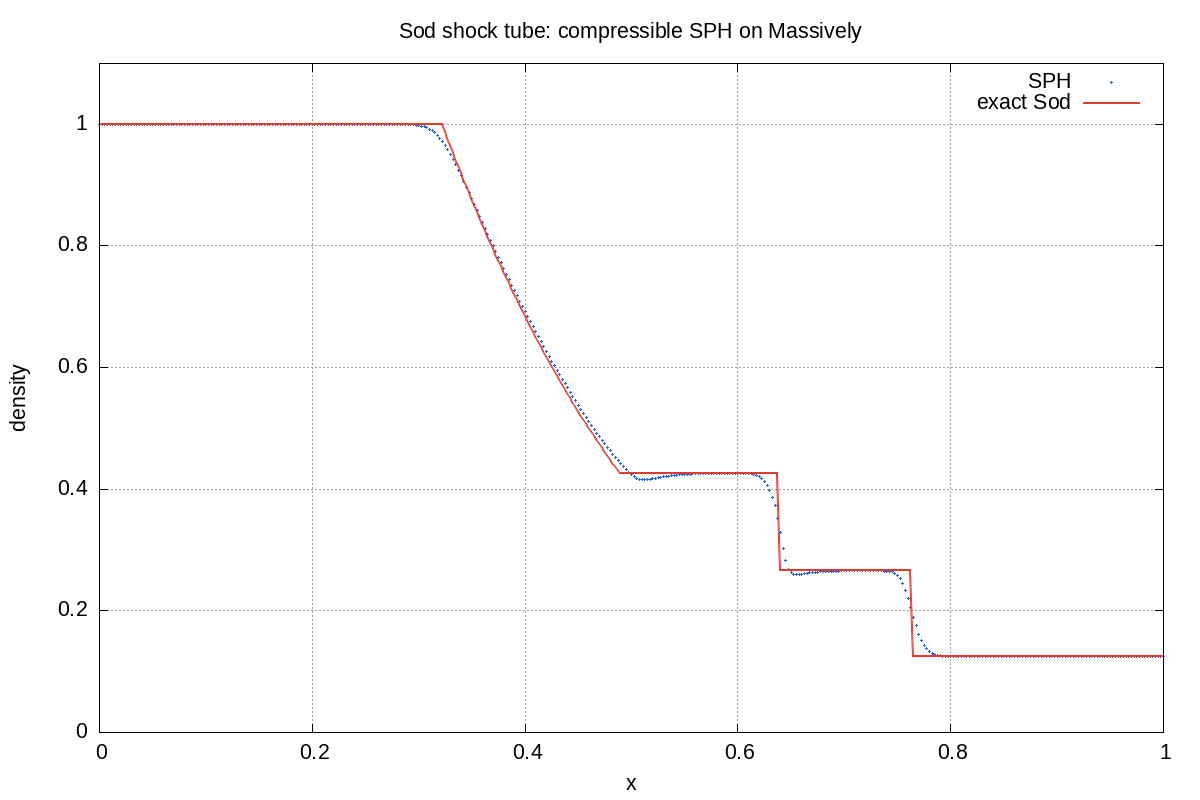
\includegraphics[width=0.88\textwidth]{shocktube.jpeg}
  \caption{$t=0.15$におけるSod shock-tube密度。GPU SPH解はrarefaction、contact
  discontinuity、shockを再現している。}
  \label{fig:shocktube-ja}
\end{figure}

Figure~\ref{fig:shocktube-ja}のsample密度の平均絶対誤差は0.00419917である。計算された最小密度は
0.124903、最小圧力は0.100179であり、全粒子質量は変化しない。plotで使用する厳密star stateは
$p_*=0.303130$、$u_*=0.927453$である。この結果は、1個の発展問題においてsort、密度、状態方程式、
圧力・粘性導関数、時間積分、およびsnapshot再構成の合成を確認する。これは収束性研究ではなく、
あらゆるSPH flow regimeを単独で検証するものでもない。

\subsection{密度pipelineの性能}

benchmarkは、内蔵Radeon 680Mを持つAMD Ryzen 7 7735U、WGPU backend、Linux 6.17、
Rust 1.96.0で実行した。GPU値とCPU cell-list値はwarm-up後の5回の計測の中央値である。GPU
snapshotにはcell-ID評価、sort、lower-bound構築、入れ子密度、状態方程式、およびsnapshotの
host転送を含む。CPU cell-listの範囲はlist構築と密度のみである。したがって、両者の時間は近傍
設計のengineering上の証拠として有用だが、state-of-the-art実装や完全なsolver stepの比較ではない。

\begin{table}[ht]
  \centering
  \caption{2次元密度benchmark（milliseconds）。}
  \label{tab:performance-ja}
  \begin{tabular}{rrrrrr}
    \toprule
    $N$ & GPU snapshot & CPU cells & CPU all pairs & CPU/GPU & 最大相対差 \\
    \midrule
     1,024 & 1.976 & 0.247 & 2.876   & 0.125 & $3.12\times10^{-7}$ \\
     4,096 & 2.018 & 0.984 & 44.764  & 0.488 & $1.61\times10^{-6}$ \\
    16,384 & 2.457 & 4.060 & 711.865 & 1.653 & $2.38\times10^{-6}$ \\
    65,536 & 5.109 & 16.204 & ---     & 3.171 & $5.89\times10^{-6}$ \\
    \bottomrule
  \end{tabular}
\end{table}

\begin{figure}[ht]
  \centering
  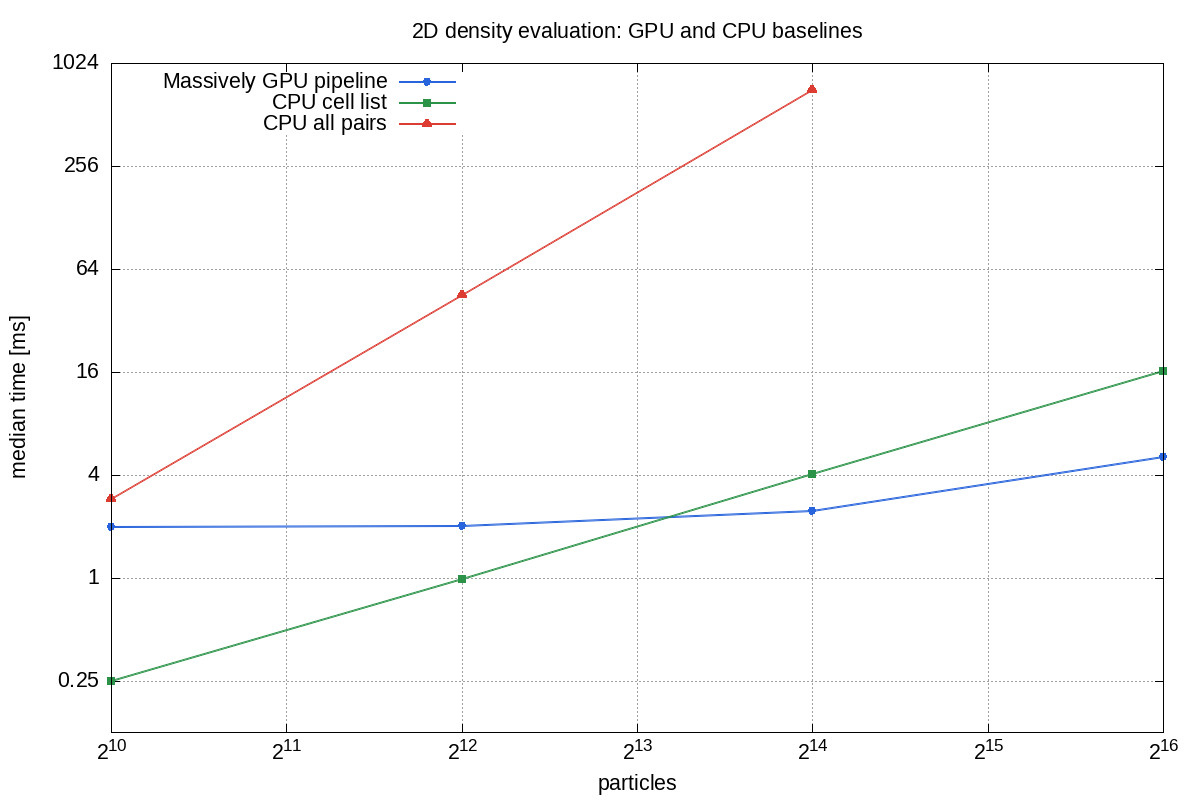
\includegraphics[width=0.96\textwidth]{performance.jpeg}
  \caption{密度pipelineのscaling。小規模入力ではdispatch overheadが支配的であり、測定した
  machineでは4,096粒子と16,384粒子の間でGPUがCPU cell実装を上回る。}
  \label{fig:performance-ja}
\end{figure}

1,024粒子では約2 msのGPU起動・同期costによりhost実装が速い。65,536粒子では、GPU snapshotが
状態方程式とhost転送を含むにもかかわらず、CPU cell-listの測定範囲より3.17倍速い。16,384粒子
では、CPU全粒子対密度はGPU snapshotより約290倍遅い。正しさについてさらに重要なのは、
全粒子対密度に対する最大相対差が最大規模でも$5.89\times10^{-6}$に留まることである。この結果は、
十分な粒子対workがあれば、入れ子viewが有用なGPU pipelineへloweringされることを示す。ただし、
sort、粒子対走査、転送の各寄与を分離した結果ではない。

\subsection{再現性}

Cargo lockfileはMassively tag v0.80のrevision
\code{f1041b5cf7902b01c303b2af3f69548e8c05cc91}を記録する。Rust workspaceのテストは
\code{cargo test --workspace}で実行する。plot scriptと生成したJPEGを\code{workspace/draw}と
\code{workspace/plot}でversion管理する。英語論文と等価な日本語論文は、宣言したDocker環境内で
\code{just --justfile paper/justfile}によりbuildし、\code{paper/paper.pdf}と
\code{paper/paper-ja.pdf}を生成する。

\section{議論と限界}

本研究の中心的な結果は表現方法である。SPHは、各粒子から近傍粒子への可変graphを必要とするように
見える。本実装が保存するのは、cellから近傍cellへの静的CSRと、cellから粒子への動的なsort済み
分割という2個の小さな関係だけである。入れ子segmentationとpermutationが、read時に両者の関係
合成を行う。これが\code{SegmentIterator}をこの問題に適合させる理由である。近傍関係をdenseで
あるかのように扱わず、別の粒子対arrayに変換することもなく、型付きiterator式を通して不揃いな
境界を運ぶことができる。

Massivelyを用いても、基礎的なcostが消えるわけではない。現在のsolverは導関数評価ごとにsortする。
粒子分布が非常に不均一ならload imbalanceが残る。gather走査は対称な粒子対workを重複させる。
13-readの境界により一部の2次元operatorは複数dispatchへ分かれる。これらは隠されたbackend詳細
ではなく、明示的な設計上のtrade-offである。

平滑化長は大域的かつ固定であり、時間積分は一次精度symplectic Euler、境界は矩形反射、
状態方程式は理想気体である。benchmarkは1個の内蔵GPUで
密度snapshotを測定したものであり、複数device上の完全な長時間simulationではない。Sodの結果は
信頼できるend-to-end baselineを確立するが、より広い数値的主張にはresolution sweepと追加の
物理問題が必要である。

実装に直接関係する次の課題は以下である。
\begin{itemize}
  \item 変位上限からcell所属が不変と証明できるsubstepでは、sort順を再利用する。
  \item 走査workの削減が追加の$O(Q)$ storageに勝る場合、Verlet候補をoptionとしてcacheする。
  \item sort、lower bound、入れ子走査、転送を個別にprofileする。
  \item vector fieldのpackingまたはMassivelyのread arity拡張により、2次元pass数を減らす。
  \item 同じCSR/segment構成を3次元へ拡張する。各rowは最大27 cellとなるため、そのcell占有数と
        divergenceを評価する。
\end{itemize}
adaptive smoothing lengthも重要な数値的拡張である。ただし、cell幅と粒子ごとのsupportを現在の
固定9-cell stencilで表せなくなるため、保守的なsupport ruleを含む新たな実装問題でもある。

\section{結論}

移動するSPH近傍は、粒子対リストを実体化せずMassively v0.80で表現できる。本実装は静的cell CSRを
保存し、全粒子columnを整合してsortし、lower boundでcell--particle offsetを導出し、遅延
permutationと2層の\code{SegmentIterator}により両関係を合成する。queryごとのgather transformが
atomic演算を不要にし、分離可能なpre/post passが完全なsolverをMassivelyの13-read型境界内に
収める。Sod shock tubeが発展solverを確認し、differential densityが近傍を全粒子対計算と照合し、
測定されたcrossoverが有用なGPU throughputを示す。同時に、繰り返すsort、対称workの重複、load
imbalance、追加passというcostを明示した。これにより、次のMassivelyおよびSPH実装を検討するための
具体的な基盤が得られた。

{\small
\bibliographystyle{plainnat}
\bibliography{references}
}

\end{document}
